\documentclass[12pt,a4paper,twoside, openright]{report}
\usepackage[utf8]{inputenc}
\usepackage{amsmath,amssymb,bm}
\usepackage{graphicx}
\usepackage{geometry}
\usepackage{fancyhdr}
\usepackage{titlesec}
\usepackage{tocloft}
\usepackage{xcolor}
\definecolor{lightgray}{gray}{0.9} % Define a light gray color
\usepackage[
colorlinks=false,        % Assign 'true' to make all links have blue font color
linkcolor=blue,    % Set internal link color to blue gray
citecolor=blue,    % Set citation link color to blue gray
urlcolor=blue,     % Set URL link color to blue gray
pdfborder={0 0 0}       % Remove borders completely
]{hyperref}
%\usepackage{mathpazo}  % Palatino font
\usepackage{setspace}  % For line spacing control
\usepackage{color,soul}  % Package for highlighting the text
\usepackage[backend=biber, style=apa, sorting=ynt, sortcites=true, apamaxprtauth=999, uniquename=false]{biblatex} % APA style with 999 max reference authors showing
\usepackage{csquotes}  % Ensure proper quoting
\addbibresource{references.bib}
\usepackage{graphicx}
\usepackage{svg}
\usepackage{float} % package is required to use the H option of figures
\usepackage{caption}   % For controlling caption spacing
\usepackage{gensymb} % for symbols
\usepackage{upgreek} % for upright greek letters
\usepackage{tabularx}
\usepackage{longtable}
\usepackage[table]{xcolor}
\usepackage{enumitem}
\usepackage{bookmark} % loads hyperref too
\usepackage{lscape}
\usepackage{diagbox}
\usepackage{booktabs}
\usepackage{array}
\usepackage[toc, acronym]{glossaries} % 
\makeglossaries

% This is to remove page numbers in blank pages, which are inserted so that the new chapters start on the right side
\makeatletter
\renewcommand{\cleardoublepage}{%
	\clearpage
	\ifodd\c@page\else
	\thispagestyle{empty}%
	\hbox{}%
	\newpage
	\fi
}
\makeatother

\setcounter{tocdepth}{3} % depth of table of contents
\setcounter{secnumdepth}{3} % This command sets the depth of section numbering

% It basically tells LaTeX that hyphenating words is a bad thing to do, but to still achieve justified paragraphs, it should just add spaces.
\tolerance=500
\emergencystretch=3em
\hyphenpenalty=5000
\hbadness=5000

\renewcommand{\floatpagefraction}{0.8}  % A float page will only be created if the floats cover at least 80% of the page. This discourages the creation of float pages with a lot of white space.
\renewcommand{\textfraction}{0.1}       % A page must have at least 10% text, which is a relatively low requirement, thereby allowing more flexibility in float placement.

% This prevents LaTeX from forcing text to spread out and instead keeps it at the top, leaving a more natural blank space at the bottom.
\raggedbottom

\captionsetup[figure]{labelsep=period, format=hang}
\captionsetup[table]{labelsep=period, format=hang}

% Decrease the space between figure and caption
\setlength{\abovecaptionskip}{5pt}   % Space above the caption
\setlength{\belowcaptionskip}{0pt}   % Space below the caption

% Set PDF metadata
\hypersetup{
	pdftitle={PhD Thesis - Savvinos Aristeidou - 2025},  % Set your desired title here
	pdfauthor={Savvinos Aristeidou},              % Set the author name
	bookmarksdepth=3  % Include up to subsubsections in bookmarks (0=chapter, 1=section, 2=subsection, 3=subsubsection)
	%	bookmarksnumbered=true,
	%	bookmarksopen=true,
	%	bookmarksopenlevel=1,
	%	pdfstartview=Fit,
	%	pdfpagemode=UseOutlines,
	%	pdfpagelayout=TwoPageRight
}

% Set margins according to the provided template
\geometry{
	top=6cm,
	bottom=4.7cm,
	inner=4cm,
	outer=3.5cm,
}

% Adjust header height
\setlength{\headheight}{14.5pt}
\addtolength{\topmargin}{-2.5pt}

% Header and Footer settings
\fancypagestyle{plain}{ % For chapters and unnumbered sections
	\fancyhf{}
	\fancyhead[RO]{\small\thepage} % Restore left header for even pages (if needed)
	\fancyhead[LE]{\small\thepage} % Restore left header for odd pages (if needed)
}

% Redefine \chapter to include \thispagestyle{empty}
\let\oldchapter\chapter
\renewcommand{\chapter}[1]{
	\oldchapter{#1}
	\thispagestyle{empty}
}

% Custom command for unnumbered chapters with header/footer clearing
\newcommand{\mychapter}[1]{ % Removed the * from here
	\oldchapter*{#1} % Call the original chapter command
	\thispagestyle{empty} % Clear the page style
	\fancyhf{} % Clear all header and footer fields
	\fancyhead[RO]{\small\thepage} % Restore left header for even pages (if needed)
	\fancyhead[LE]{\small\thepage} % Restore left header for odd pages (if needed)
}

% Redefine section and chapter titles
\titleformat{\chapter}[display]
{\normalfont\LARGE\bfseries}{\chaptertitlename\ \thechapter}{20pt}{\LARGE}


% Page numbers in Roman numerals for front matter pages
\pagenumbering{roman}

\newacronym{GGMM}{GGMM}{generalised ground motion model}
\newacronym{GMM}{GMM}{ground motion model}
\newacronym{IM}{IM}{intensity measure}
\newacronym{NGA-West2}{NGA-West2}{next generation attenuation relationships for Western United States}
\newacronym{SDOF}{SDOF}{single-degree-of-freedom}
\newglossaryentry{Ds}{
	name=\ensuremath{Ds},
	description={significant duration},
	sort={Ds},
	first={significant duration, $Ds$}
}
\newglossaryentry{FIV3}{
	name=\ensuremath{FIV3},
	description={filtered incremental velocity},
	sort={FIV3},
	first={filtered incremental velocity, $FIV3$}
}
\newglossaryentry{PGA}{
	name=\ensuremath{PGA},
	description={peak ground acceleration},
	sort={PGA},
	first={peak ground acceleration, $PGA$}
}
\newglossaryentry{PGV}{
	name=\ensuremath{PGV},
	description={peak ground velocity},
	sort={PGV},
	first={peak ground velocity, $PGV$}
}
\newglossaryentry{Sa}{
	name=\ensuremath{Sa},
	description={5\% damped spectral acceleration},
	sort={Sa},
	first={spectral acceleration, $Sa$}
}
\newglossaryentry{Saavg}{
	name={$Sa_\text{avg}$},
	description={average spectral acceleration},
	sort={Saavg},
	first={average spectral acceleration, $Sa_\text{avg}$}
}
\newglossaryentry{Saavg3}{
	name={$Sa_\text{avg3}$},
	description={average spectral acceleration over the period range [0.2$T$, 3$T$]},
	sort={Saavg3},
}








\begin{document}
	
	% Savvinos: I changed the title according to your suggestion. Sounds good for now!
	% Title Page
	\begin{titlepage}
		\centering
		\begin{figure}[h!]
			\centering
			
\includegraphics[width=0.8\textwidth]{figures/IUSS_logo.png}
		\end{figure}
		\text{Scuola Universitaria Superiore IUSS Pavia}\\
		\vspace*{2cm}
		{\Large\bfseries ADVANCES IN THE PRACTICAL APPLICATION OF NEXT-GENERATION INTENSITY MEASURES FOR EFFICIENT SEISMIC RISK ASSESSMENT\par}
		\vspace{1cm}
		\textit{A Thesis Submitted in Partial Fulfilment of the Requirements\\
			for the Degree of Doctor of Philosophy in}\\[1cm]
		\textbf{EARTHQUAKE ENGINEERING AND ENGINEERING SEISMOLOGY}\\
		\vspace{1cm}
		\textit{Obtained in the framework of the Doctoral Programme in}\\[0.8cm]
		\textbf{Understanding and Managing Extremes}\\[1cm]
		\textit{by}\\[0.3cm]
		\textbf{Savvinos Aristeidou}\\
		\vfill
		\textit{May 2025}
	\end{titlepage}
	
	\cleardoublepage % Ensures the next title page starts on a right-hand page

	
	% Second title Page
	\begin{titlepage}
		\centering
		\begin{figure}[h!]
			\centering
			
\includegraphics[width=0.8\textwidth]{figures/IUSS_logo.png}
		\end{figure}
		\text{Scuola Universitaria Superiore IUSS Pavia}\\
		\vspace*{2cm}
		{\Large\bfseries ADVANCES IN THE PRACTICAL APPLICATION OF NEXT-GENERATION INTENSITY MEASURES FOR EFFICIENT SEISMIC RISK ASSESSMENT\par}
		\vspace{1cm}
		\textit{A Thesis Submitted in Partial Fulfilment of the Requirements\\
			for the Degree of Doctor of Philosophy in}\\[1cm]
		\textbf{EARTHQUAKE ENGINEERING AND ENGINEERING SEISMOLOGY}\\
		\vspace{1cm}
		\textit{Obtained in the framework of the Doctoral Programme in}\\[0.8cm]
		\textbf{Understanding and Managing Extremes}\\[1cm]
		\textit{by}\\[0.3cm]
		\textbf{Savvinos Aristeidou}\\[0.3cm]
		\text{Supervisor: Prof. Gerard O'Reilly}\\
		\vfill
		\textit{May 2025}
	\end{titlepage}
	
	% Header and footer for main document
	\pagestyle{fancy}
	\fancyhf{}
	\fancyhead[RO]{\small\thepage} % Restore left header for even pages (if needed)
	\fancyhead[LE]{\small\thepage} % Restore left header for odd pages (if needed)
	
	% Gerard O'Reilly: It is a little segmented because you were aggregating the existing abstracts from past papers, but otherwise it is fine I think
	% Abstract
	\oldchapter*{Abstract}
	\addcontentsline{toc}{chapter}{Abstract}
	
	This report contains guidelines for formatting a PhD Thesis.
	
	\newpage
	
	% Abstract in italian
	\oldchapter*{Sommario}
	\addcontentsline{toc}{chapter}{Sommario}
	
	Questo rapporto contiene le linee guida per la formattazione di una tesi di dottorato.

	\newpage
	
	% Acknowledgements
	\oldchapter*{Acknowledgements}
	\addcontentsline{toc}{chapter}{Acknowledgements}
	
	Acknowledgements can be provided here (though it is not compulsory to include them).

	\newpage
	
	%\hypertarget{toc}{}% set the hypertarget
	%\bookmark[dest=toc,level=chapter]{\contentsname}% add the bookmark
	
	\glsunsetall  % Disable all expansions of abbreviations and symbols
	
	% Table of Contents
	\phantomsection   % Creates an invisible anchor for hyperlinking
	\addcontentsline{toc}{chapter}{Contents}
	\tableofcontents
	
	\newpage
	
	% List of Figures
	\phantomsection   % Creates an invisible anchor for hyperlinking
	\addcontentsline{toc}{chapter}{List of Figures}
	\listoffigures
	
	\newpage
	
	% List of Tables
	\phantomsection   % Creates an invisible anchor for hyperlinking
	\addcontentsline{toc}{chapter}{List of Tables}
	\listoftables
	
	\newpage
	
	\glsresetall  % Re-enable expansions of abbreviations and symbols
	
	\oldchapter*{Nomenclature}
	\addcontentsline{toc}{chapter}{Nomenclature}
	
	\section*{List of abbreviations}
	
	\vspace{-1cm} % Adjust the value as needed
	% Prevents LaTeX from inserting a new chapter
	\renewcommand*{\glossarysection}[2][]{\section*{#2}}
%	\glsaddall
	\printglossary[type=\acronymtype, title={}, toctitle={}, style=long, nogroupskip, nonumberlist]
	
%	% Set the vertical space between rows
%	\renewcommand{\arraystretch}{1.5} % Adjust this value for desired spacing
	
	\section*{List of symbols}
	
	\vspace{-1cm} % Adjust the value as needed
	\printglossary[title={}, toctitle={}, style=long, nogroupskip, nonumberlist]
%	\printglossary[title={List of Symbols}]
	
	
	\renewcommand{\arraystretch}{1.2} % Reset to default (actually a little higher for table clarity)
	
	\cleardoublepage
	
	% Header and footer for main document
	\pagestyle{fancy}
	\fancyhf{}
	\fancyhead[RE]{\small\nouppercase{\leftmark}} % Left header on even pages: Chapter title
	\fancyhead[RO]{\small\thepage}  % Right header on even pages: Page number
	\fancyhead[LO]{\small Savvinos Aristeidou} % Right header on odd pages: Author's name
	\fancyhead[LE]{\small\thepage}  % Left header on odd pages: Page number
	
	% Switch to Arabic numerals for Chapter 1 onwards
	
	\pagenumbering{arabic}
	
	 \chapter{Guidelines for the PhD thesis}
\label{chapter:guidelines}

This chapter is extensively based on the following publication:\\
\\
\fullcite{Aristeidou2023}

% NOTE: Acronyms are defined only in abstract, introduction and conclusions chapters.

\section{Introduction}

Please read carefully the instructions presented herein for the format of a PhD thesis at IUSS Pavia. This document was written to be loosely based on the required format, therefore please read the document for any formatting requirements that are not explicitly stated in the text. Any formatting styles not described herein are either coded in the preamble, or are left to the author's discretion.

\section{General settings}

The page setup options are in the preamble of ``\texttt{main.tex}" file and described in the following. The margins for A4 size paper should be fixed as: top 6cm, bottom 4.7cm, inside 4cm and outside 3.5cm. The page margins should be mirrored. New chapters should start on odd page numbers and the headers are different on odd and even pages. The header and footer should be set at 4.8cm and 1.5cm from edge, respectively. It must be ensured that first page of each chapter is located on the right-hand side of the double-sided document.

\section{Formatting and styling}

The formatting settings are already implemented in the LaTex files. Nevertheless, they are also summarised along the text herein. All the styles are set in the preamble.

\subsection{The body text}

The language of the main text should be set to English (United Kingdom). Abbreviations are allowed but should be spelt out in full when first used in the abstract, introduction, and conclusions chapters. Integers from one to ten should be written out in words. Foreign language phrases should be italicised (e.g., Latin, French).

\subsection{Header and page numbering}

The header should vary for the first, odd and even pages: there should be no header on the first page of each section/chapter, on even pages the title of the chapter should be inserted (it is automatically reported if added in the first page of the chapter), whilst the name of the author should be placed on the header of odd pages. The text size of headers and page numbers is ``\textbackslash small". Page numbers should be flush outside on odd pages and flush inside on even pages. The preliminary pages of the thesis from the Abstract to the last page of the Nomenclature should be numbered using Roman numerals (i.e. i, ii, iii).  The page numbers should restart using Arabic numbers (i.e. 1, 2, 3) on the first page of Chapter \ref{chapter:guidelines} and should continue until the last page of the report/thesis.

It is worth mentioning that the user can modify the font style of the document and the template will be completely updated.

\subsection{Equations, figures and tables}

Equations should be centred within the text width, whilst equation numbers should be placed in parentheses and set flush with the right margin, as illustrated in Equations \ref{median_GCIM} and \ref{sigma_GCIM}.

\begin{equation}
	\mu_{\ln \text{IM}_\text{i} | \ln \text{IM*}, \text{rup}} = \mu_{\ln \text{IM}_\text{i} | \text{rup}} + \sigma_{\ln \text{IM}_\text{i} | \text{rup}} \cdot \rho_{\ln \text{IM}_i, \ln \text{IM*}} \cdot \epsilon_{\ln \text{IM*}}
	\label{median_GCIM}
\end{equation}

\begin{equation}
	\sigma_{\ln \text{IM}_\text{i} | \ln \text{IM*}, \text{rup}} = \sigma_{\ln \text{IM}_\text{i} | \text{rup}} \cdot \sqrt{1 - \rho_{\ln \text{IM}_\text{i}, \ln \text{IM*}}^2}
	\label{sigma_GCIM}
\end{equation}

In equations, the text, variables and functions should be in \textit{Italic}, whilst numbers, functions and subscripts should not. The sequence of braces, brackets, and parentheses in equations should generally be $\{[( )]\}$, with due consideration given to the specific meanings associated with different types of brackets.

Figures should be included in the report as illustrated in Figure \ref{IUSS_logo}; there should be 3pt space before and 6pt space after each figure. A caption should be inserted using the pre-defined format in the preamble. The captions of figures should be centred.

\begin{figure}
	\centering
	
\includegraphics[width=0.6\textwidth]{figures_ch1/IUSS_logo.png}
	\caption{Example figure}
	\label{IUSS_logo}
\end{figure}

Tables should have the format shown in Table \ref{tab:modal_analysis}. The captions of tables should be centre-aligned and justified (as in Table \ref{tab:modal_analysis}). Titles of the cells should be in bold font, and for the contents a smaller font size may be used (e.g., ``\textbackslash small").

\begin{table}
	\centering
	\caption{Modal analysis results of the case study bridge.}
	\begin{tabularx}{\textwidth}{ccXXXXXX}
		\hline
		& & \multicolumn{6}{c}{\textbf{Modal participation mass ratios [\%]}} \\ \cline{3-8}
		\textbf{Mode} & \textbf{Period [sec]} & $\bm{U_x}$ & $\bm{U_y}$ & $\bm{U_z}$ & $\bm{\Phi_x}$ & $\bm{\Phi_y}$ & $\bm{\Phi_z}$ \\ \hline
		1 & 0.604 & 48.5 & 0 & 0 & 0 & 31.1 & 0 \\
		2 & 0.363 & 50.5 & 0 & 0 & 0 & 34.6 & 0 \\
		3 & 0.352 & 0 & 88.3 & 0 & 0.5 & 0 & 0 \\
		4 & 0.336 & 0 & 0 & 75.4 & 0 & 0 & 0 \\ \hline
	\end{tabularx}
	\label{tab:modal_analysis}
\end{table}

\subsection{References}

All references should be cited in the text by name and year and may take one of the following forms: ``…as shown by \textcite{Tarbali2019}, the…" or ``…has often been demonstrated \parencite{Davalos2020b, Davalos2019, Aristeidou2024a} that…" The reference list should be placed at the end of the thesis, but before the appendices (if any), and must be in alphabetical order by first authors' surnames and presented in the style shown in the examples in the reference section of these guidelines.

\subsection{Appendices}

Any appendices included in the document should be numbered alphabetically and placed at the end of the thesis after the references (see example at the end of this document).
 % Include chapter_1.tex
	
	 \chapter{Example second chapter}
\label{chapter:second_ch}

This chapter is extensively based on the following publication:\\
\\
\fullcite{Aristeidou2024c}

\section{Introduction}

Example figures are shown in Figures \ref{sdof_bilinear_model} and \ref{Saavg3_FIV3_empirical_predicted_total_correlation}, inserted from a pdf file and svg file, respectively.

\begin{figure}
	\centering
	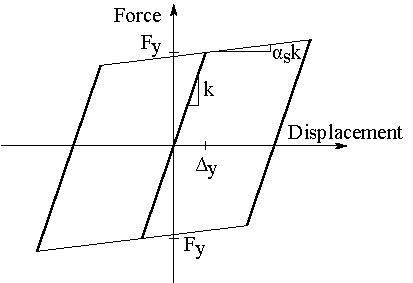
\includegraphics{figures_ch2/sdof_bilinear_model.pdf} % didn't specify width here
	\caption{Hysteretic behaviour of the bilinear \gls{SDOF} model (inserted from a pdf file)}
	\label{sdof_bilinear_model}
\end{figure}

\begin{figure}
	\centering
	\includesvg[width=1\textwidth]{figures_ch2/Saavg3_FIV3_empirical_predicted_total_correlation.svg}
	\caption{Empirical and corresponding predicted correlation coefficients between \gls{Saavg3} and \gls{FIV3} (inserted from an svg file)}
	\label{Saavg3_FIV3_empirical_predicted_total_correlation}
\end{figure}

\section{Discussion and conclusions}

This study presented the empirical correlations between assorted \glspl{IM} of various types, namely \gls{PGA}, \gls{PGV}, \gls{Sa}, \gls{Ds}, \gls{Saavg}, and \gls{FIV3}. The residuals, which are used for the calculation of correlations, were obtained from a previously developed \gls{GGMM} and the same filtered ground motion database. This is believed to produce more consistent correlation coefficients since the same database subset is used for the development of the \gls{GMM} and the calculation of empirical correlation coefficients.


 % Include chapter_2.tex
	
	% References
	\mychapter{References}
	\addcontentsline{toc}{chapter}{References}
	\thispagestyle{empty}
	
	%\printbibliography[heading=none]
	\begin{refcontext}[sorting=nyt]
		\printbibliography[heading=none]
	\end{refcontext}
	
	\newcommand{\AppendixATitle}{Appendix A. Influence of database subset selection on correlation coefficients}
	\oldchapter*{\AppendixATitle}
	\addcontentsline{toc}{chapter}{\AppendixATitle}
	\label{Appendix A}
	\renewcommand{\thefigure}{A.\arabic{figure}}
	
	This appendix briefly examines what is the main cause of difference between the cross-correlation coefficients proposed here and the ones available in the literature. With that, more general conclusions can be outlined on the importance of different decisions when developing correlation models.
	
	In Figure \ref{Sa_Sa_total_correlation_comparison_slices_nga_west} four different \gls{NGA-West2} \glspl{GMM} were used with the same filtering criteria. The filtering criteria are the ones actually used in this study. It can be clearly seen that the correlations obtained from the different \glspl{GMM} give very similar results. Therefore, we can safely say that the correlation results are not biased by the use of a single \gls{GMM} and that the ASO24 model is also in line with the others.
	
	The same records and same \gls{GMM} as BB17 was used to calculate the correlations and compared with the BB17 model itself in Figure \ref{Sa_Sa_total_correlation_comparison_slices_diff_filt}. The BB17 model used the \gls{NGA-West2} database and is very close to BJ08 model. The results, as expected, are very close. The figures in this appendix constitute strong evidence that the difference comes from the filtering (i.e., subset selection) of the database and not from the background \gls{GMM} adopted.
	
	\begin{figure}
		\centering
		\includesvg[width=0.8\textwidth]{figures_appendix/Sa_Sa_total_correlation_comparison_slices_nga_west.svg}
		\caption{Comparison of correlation coefficients derived from utilising each of the four \gls{NGA-West2} \glspl{GMM} and the one employed for this study}
		\label{Sa_Sa_total_correlation_comparison_slices_nga_west}
	\end{figure}
	
	\begin{figure}
		\centering
		\includesvg[width=1\textwidth]{figures_appendix/Sa_Sa_total_correlation_comparison_slices_diff_filt.svg}
		\caption{Correlations proposed by BB17, and the ones calculated here with the same \gls{GMM} (i.e., CY14) and the same ground motion records}
		\label{Sa_Sa_total_correlation_comparison_slices_diff_filt}
	\end{figure}
	
	
\end{document}
